\chapter{Grundlagen} % und verwandte Arbeiten
\label{ch:background}
Das Ziel von \ac{bi} ist es, aus operativen und externen Daten Informationen und aus diesem Wissen zu gewinnen. Damit ist es ein wertvolles Werkzeug zur Entscheidungshilfe und Planung. Prozesse zur Beschaffung, Transformation, Aufbereitung, Speicherung und Analyse von Daten, aber auch die Qualitätssicherung, sind Bestandteile eines BI-Systems \cite{muller_business_2013}. Ein BI-System kann in vier oder fünf grundlegende Bestandteile aufgeteilt werden. Die \textit{Datenversorgung} ist zuständig für den Zugriff auf verschiedene Datenquellen. Dabei können die Daten transformiert, aggregiert, bereinigt und auf Plausibilität geprüft werden. Die Speicherung der Daten fällt unter das \textit{Datenmanagement}. Anwendungen zur Aufbereitung und Darstellung dieser Daten gehören zu den \textit{BI-Anwendungen}. Im \textit{Metadatenmanagement}, werden relevante Metadaten, wie Zugriffsrechte oder Informationen zu dem Quellsystem verwaltet \cite{kemper_bi-glossar_2008}. Beim \textit{Warehouse Management} handelt es sich um die Verwaltung und Wartung der gesamten BI-Infrastruktur \cite{grunwald_business_2009}. Dazu zählt unter anderem die Überwachung der Systemauslastung und das Installieren von Softwareupdates. Das {Metadatenmanagement} wird nicht immer als eigener Bestandteil angesehen, sondern häufig als Teil des {Warehouse Managements} \cite{humm_architektur_2005}. So wird das {Metadatenmanagement} auch im Folgenden betrachtet.


\section{Beschreibung der aktuellen on-premise BI-Architektur} \label{sec:grundlagen:onpremiseBI}
Die Ausgangslage für die Migration ist ein on-premise betriebenes BI~=System. Dieses ist in der \textit{Hub~=and~=Spoke-Architektur} aufgebaut. Diese gängige Architektur beschreibt die Verwendung eines zentralen Datenspeicherorts (Hub) und darauf aufbauenden, für bestimmte Auswertungen oder Anwendungen optimierte, Datenspeicher (Spokes) \cite{kemper_bi-glossar_2008}. Die Daten aus dem Hub werden also weiterverarbeitet und in den spezialisierten Spokes abgelegt. Abbildung~\ref{fig:aktuelle_onpremise_bi_architektur} zeigt die aktuelle BI~=Architektur, aufgeteilt nach funktionalen Bereichen.
\begin{figure}[htbp]
 \centering
 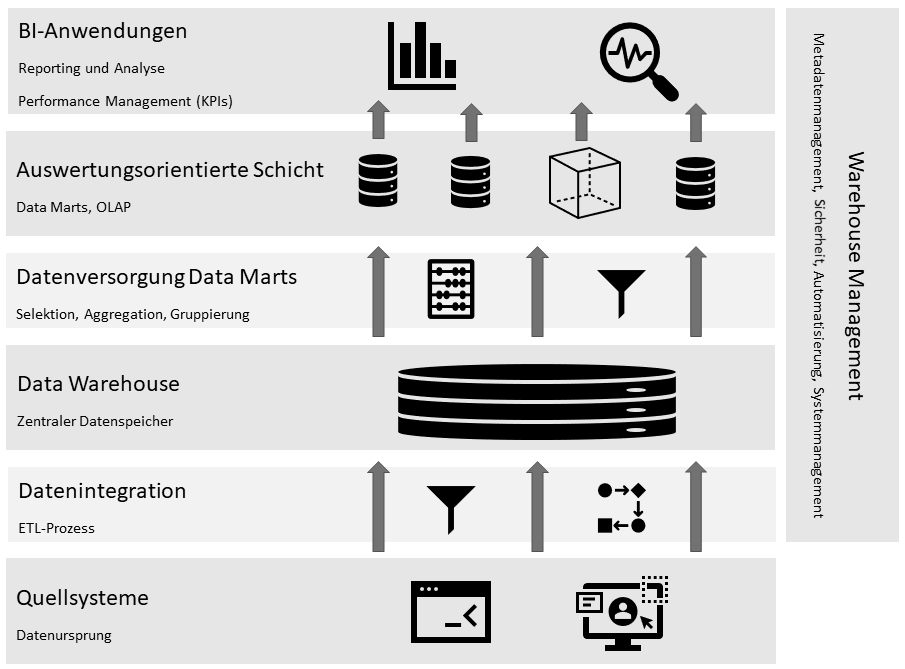
\includegraphics[width=\textwidth]{gfx/aktuelle_onpremise_bi_architektur.png}
 \caption{Aktuelle Architektur des on-premise BI-Systems und Ausgangslage für die Migration in die Cloud \cite{grunwald_business_2009}\cite{humm_architektur_2005}}
\label{fig:aktuelle_onpremise_bi_architektur}
\end{figure}
Die einzelnen Schichten werden im Folgenden erläutert \cite{grunwald_business_2009}\cite{kemper_bi-glossar_2008}\cite{humm_architektur_2005}:
\begin{itemize}
\item \textbf{Quellsysteme} sind der Ursprung aller Daten des BI-Systems. Es kann sich hierbei um interne, sowie externe Quellen handeln. Externe Daten könnten beispielsweise von Marktforschungs- oder Partnerunternehmen stammen. Aktuell sind nur interne Datenquellen angeschlossen. Darunter zum Beispiel die Projektmanagement-Software Jira und das Codeanalyse-Tool SonarQube.
\item Die \textbf{Datenintegration}(\ac{etl}) ist die Schnittstelle zwischen dem \ac{dwh} und den Quellsystemen. Der \acs{etl}-Prozess beginnt mit dem Extrahieren von operativen Daten aus einem Quellsystem. Darauf folgt eine Transformation, bei der die Daten an syntaktische Anforderungen angepasst werden und semantische Fehler, wenn möglich, behoben werden. Abschließend werden die Daten in das \ac{dwh} zur Speicherung geladen. Für den \acs{etl}-Prozess werden Funktionen von \textit{Microsofts SQL Server} und \textit{Powershell-Skripte} genutzt.
\item Das \textbf{Data Warehouse} ist der zentrale Speicherort. Hier werden die Daten strukturiert und langfristig abgelegt. Damit werden sie für weitere Verarbeitungsschritte und Auswertungen zur Verfügung gestellt. In diesem BI-System wird für das Data Warehouse das relationale Datenbankmanagementsystem \textit{Microsoft SQL Server} verwendet.
\item \textbf{Datenversorgung Data Marts}: Durch den Einsatz von SQL werden in dieser Schicht Bereich Daten selektiert, gruppiert und aggregiert. Das Ziel ist die Aufbereitung der Daten für die Data Marts.
\item \textbf{Auswertungsorientierte Schicht}: Data Marts beinhalten spezialisierte Ausschnitte der Daten aus dem \ac{dwh}, in einer für den Zugriff aus den BI-Anwendungen optimierten Form. Ziel ist es, dass für alle Anwendungsfälle eine effiziente Auswertung ermöglicht wird. Verschiedene Data Marts greifen beispielsweise auf die gleichen Daten mit unterschiedlichem Detailgrad und Selektionskriterien zu. Für komplexere Datenanalysen wird das Konzept des \textit{\ac{olap}} angewendet. Dieses soll es Nutzern ermöglichen, auch ohne technische Kenntnisse, Wissen aus dem \ac{dwh} oder den Data Marts zu extrahieren. Das kann durch die Bereitstellung von Ad-hoc-Reports geschehen, welche eine Benutzeroberfläche besitzen, über die mit einfachen Interaktionen flexible Analysen durchgeführt werden können. Dadurch sind keine Kenntnisse in einer Datenbankabfragesprache, wie SQL, notwendig. Die Grundlage für das \ac{olap} sind die sogenannten \ac{olap} Cubes. Unter diesen wird ein multidimensionaler Datenraum verstanden, bei dem die Dimensionen verschiedenen Kontexte, wie zum Beispiel Produkte, Kunden oder Zeit beschreiben. Sowohl die Data Marts als auch die \ac{olap} Cubes sind entweder als View auf das \ac{dwh} oder als eigenständige Datenbanktabelle realisiert.
\item \textbf{BI-Anwendungen} sind die Benutzerschnittstelle zum BI~=System. Hier erfolgen Auswertung und Präsentation. Im aktuellen BI~=System existieren drei Reporting-Anwendungen, die jeweils eine andere Management~=Ebene als Zielgruppe haben. Von den verschiedenen Arten an BI~=Anwendungen werden die Kategorien \textit{Reporting und Analyse} und \textit{Performance Management} abgedeckt. Bei der ersten Kategorie werden standardisierte Berichte in Form von Listen, Tabellen und Grafiken zur Verfügung gestellt. Beim {Performance Management} wird die Unternehmensleistung anhand von ausgewählten \acp{kpi} dargestellt und mit Zielwerten verglichen. Die vorhandenen BI-Anwendungen wurden mit einem internen Reporting~=Framework entwickelt, das auf dem Web~=Framework AngularJS und einer Java"-script Bibliothek zum Erstellen von Visualisierungen basiert.
\item Das \textbf{Warehouse Management} umfasst Aufgaben bezüglich Aufbau, Pflege und Betrieb des BI-Systems:
\begin{itemize}
\item \textit{Metadatenmanagement}. Verwaltung von Metadaten und Bereitstellung einer gemeinsamen Metadatenbasis für alle Komponenten im System.
\item \textit{Sicherheit}. Authentifizierung und Autorisierung von Benutzern.
\item \textit{Automatisierung}. Event- oder zeitbasierte Ausführung von Prozessen im \ac{dwh}. Zum Beispiel das Ausführen eines ETL-Prozesses zu einer festen Uhrzeit.
\item \textit{Systemmanagement}. Betrieb des \ac{dwh}s gewährleisten. Dazu gehört zum einen die Überwachung von Performance und Auslastung des Systems und zum anderen die Archivierung und Sicherung von Daten.
\end{itemize}
\end{itemize}

\section{Business Intelligence in der Azure Cloud} \label{sec:grundlagen:bi_in_der_cloud_mit_azure}
In der Cloud wird eine Vielzahl an Ressourcen, wie virtualisierte Hardware oder Dienste, zur Verfügung gestellt. Diese können dynamisch konfiguriert und skaliert werden, sodass immer die benötigte Leistung zur Verfügung steht. Microsoft Azure ist eine Sammlung an solchen Ressourcen, die sich aktuell in 22 Kategorien einteilen lassen. Manche Dienste können dabei zu mehreren Kategorien gehören. Für den Entwurf der neuen BI-Architektur werden Dienste aus den folgenden Kategorien in Betracht gezogen \cite{chilberto_building_2020}:
\begin{itemize}
\item \textbf{Integrations}~=Dienste können eingesetzt werden, um die Daten aus Cloud und on-premise Anwendungen zu laden.
\item \textbf{Datenbank}~=Dienste sind unter anderem relationale Datenbanken, wie Azure SQL, MySQL und PostgreSQL. Eine Alternative dazu ist die NoSQL-Datenbank Azure Cosmos DB, welche mehrere Datenmodelle unterstützt.
\item \textbf{Speicher}-Dienste sind in verschiedenen Ausprägungen vorhanden und können nach den individuellen Anforderungen ausgewählt werden. Ziel ist es, eine große Menge an Daten, die sowohl strukturiert als auch unstrukturiert sein kann, möglichst günstig abzuspeichern.
\item \textbf{Analyse}-Dienste helfen, die benötigten Erkenntnisse aus den Daten zu gewinnen.
\item \textbf{KI und Machine Learning} ermöglicht komplexere Analysen. Zum Beispiel können, basierend auf historischen Daten, Vorhersagen über die Zukunft getroffen werden. Diese können beispielsweise genutzt werden, um die zukünftige Entwicklung von KPIs abzuschätzen.
\item \textbf{Identitäts}-Dienste werden genutzt, um sicherzustellen, dass nur berechtigte Nutzer Zugriff auf Anwendungen und Daten erhalten.
\item \textbf{Netzwerk}-Dienste werden verwendet, um eine sichere Verbindung zwischen on-premise und Cloud Infrastruktur herzustellen.
\item \textbf{Sicherheit} ist ein wichtiges Kriterium für Cloud-Systeme. Azure stellt hierfür Dienste zur Überwachung der Datensicherheit und zum Erkennen von Sicherheitsrisiken bereit.
\item \textbf{Verwaltung und Governance} umfasst Dienste zur Automatisierung, sowie zur Verwaltung und Überwachung der Cloud-Ressourcen. Dazu gehört das Erstellen von Backups, sowie das Monitoring von Anwendungen, der Infrastruktur und den dadurch entstehenden Kosten.
\item \textbf{Migrations}-Dienste sollen beim Umstieg von on-premise zu Cloud Ressourcen unterstützen. Sie könnten zum Beispiel eingesetzt werden, um Daten aus dem bestehenden \ac{dwh} in eine Cloud Alternative zu übertragen.
\end{itemize}
Beim Vergleich der Azure Kategorien mit den funktionalen Schichten des on-premise BI-Systems decken die \textit{Integrations-Dienste} die  Funktionalität der \textit{Datenintegration} ab. Das \ac{dwh} kann in Azure entweder mit den \textit{Datenbank-}, den \textit{Speicher-Diensten} oder einer Kombination von beiden ersetzt werden. Die \textit{Analyse-Dienste} entsprechen der \textit{auswertungsorientierten Schicht} und den \textit{BI-Anwendungen} des on-premise Systems. Zusätzlich neue Auswertungsmöglichkeiten bieten die Dienste aus \textit{KI und Machine Learning}. Die Kategorien \textit{Identität}, \textit{Netzwerk}, \textit{Sicherheit} und \textit{Verwaltung und Governance} sind vergleichbar mit dem \textit{Warehouse Management}.

\section{Azure Dienste} \label{sec:grundlagen:azure_dienste}

\subsection{Azure SQL} \label{sec:grundlagen:azure_dienste:sql}
Azure SQL ist eine relationale Datenbank, die vergleichbar mit dem on-premise Microsoft SQL Server, der im aktuellen BI-System genutzt wird, ist. Bei einer Migration hat dies den Vorteil, dass die meisten SQL-Queries zum Laden und Transformieren von Daten, ohne Anpassung verwendet werden können. Der Einsatz von Azure SQL empfiehlt sich besonders, wenn hochgradig relationale Daten vorliegen \cite{reagan_azure_2018}. 

Die alternativen relationalen Datenbanken in Azure, wie MySQL und PostgresSQL, werden in dieser Arbeit nicht betrachtet.

\subsection{Azure Table Storage} \label{sec:grundlagen:azure_dienste:tableStorage}
Der NoSQL-Dienste Azure Table Storage gehört zu den günstigsten Speichermöglichkeiten in Azure. Die Daten werden als Schlüssel/Wert-Paare in Tabellen gespeichert, diese sind jedoch nicht relational und können nicht miteinander gejoint werden. Eine Tabelle besteht aus einer oder mehreren Partitionen und eine Partition besteht aus ein oder mehreren Zeilen. Auf jeden Tabelleneintrag kann über einen eindeutigen Schlüssel zugegriffen werden. Dieser ist eine Kombination aus Partitions- und Zeilen-Schlüssel. Die Partitionierung über mehrere Server ermöglicht es Datenmengen im dreistelligen Terabyte Bereich zu speichern \cite{reagan_azure_2018}. 

\subsection{Azure Cosmos DB} \label{sec:grundlagen:azure_dienste:cosmosDB}
Bei diesem Dienst handelt es sich um eine Datenbank, die mehrere Datenmodelle, wie Schlüssel-Wert, Dokument oder Graph, unterstützt. Eines der Features ist die automatisierbare Replikation über verschiedene Regionen. Dadurch können weltweit geringe Latenzzeiten gewährleistet werden. Die \acp{sla} sichern außerdem eine Verfügbarkeit von 99,99\% zu \cite{guay_paz_introduction_2018}. 

\subsection{Azure Data Lake Gen 2} \label{sec:grundlagen:azure_dienste:dataLake}
\acp{blob} sind unstrukturierte Dateien, die sich nicht zum Speichern in einer Datenbank eignen. Eine kostengünstige Möglichkeit, diese in der Cloud abzulegen, ist der Azure Blob Storage. Auf diesen Dienst baut auch der Azure Data Lake Gen 2 auf, welcher für die Analyse der gespeicherten Daten spezialisiert wurde \cite{soh_azure_2020}.

\subsection{Azure Data Factory} \label{sec:grundlagen:azure_dienste:dataFactory}
Azure Data Factory ist ein Datenintegrationsdienst, der für on-premise und Cloud Systeme genutzt werden kann. Der Dienst wurde speziell für den gemeinsamen Einsatz mit anderen Diensten entwickelt und übernimmt dabei die Bewegung, Transformation und Verarbeitung der Daten, zwischen den unterschiedlichen Systemen \cite{klein_azure_2017}.

\subsection{Azure Synapse Analytics} \label{sec:grundlagen:azure_dienste:synapseAnalytics}
Azure Synapse Analytics vereint die Datenintegration, Data Warehousing und Big Data Analysen zu einem Dienst. Die Datenintegration verwendet die Azure Data Factory, wird hier aber als \textit{Synapse Pipeline} bezeichnet. Die integrierten Daten können unabhängig von ihrer Struktur gespeichert werden. Durch die Unterstützung von Apache Spark wird die Analyse von großen Datenmengen ermöglicht \cite{shiyal_beginning_2021}. 
